%!TEX encoding = UTF-8

\chapter{Background}
\label{chap:background}

In this chapter, we provide the theoretical groundwork for the thesis.
In Sec.~\ref{sec:background:theory} we define some necessary machine learning concepts and models, how to train these models and how to make use of them.
Then, in Sec.~\ref{sec:background:previous_works} we discuss the main works in the literature which are related to the broad scope of the thesis~(note that, in the other chapters, we will also provide chapter-specific summaries of the related works about a particular topic, for example tool use in robotics).

\section{Theoretical Concepts}
\label{sec:background:theory}

In this section, we introduce the probabilistic models and machinery used for developing affordance learning in the rest of the thesis.
We adopt the notation from~\cite{bishop:prml}.

\subsection{Probability Theory}
\label{sec:background:theory:probability}

A random variable~$X$ is a variable whose possible values are numerical outcomes of a random phenomenon.
In general, these outcomes can be discrete or continuous, but \emph{we focus on random variables with discrete values}.
We write~$p(X = x_i)$ (supposing discrete values indexed by~$i = 1, \dots, M$) to denote the probability that~$X$ takes the value~$x_i$.
Given two random variables~$X$ and~$Y$, the notation $p(X=x_i, Y=y_j)$ indicates the \emph{joint probability} of~$X = x_i$ and~$Y = y_j$ ($j = 1, \dots, L$), expressing the probability that each of~$X$ and~$Y$ falls in any particular value specified for that variable.
In the case of two random variables, this joint probability distribution is also called a bivariate distribution.
The concept can be generalized to any number of random variables: in that case, it is called a multivariate distribution.

The joint probability distribution can be used to determine two other types of distributions:
\begin{itemize}
    \item the \emph{marginal probability} distribution, which gives the probabilities for any one of the variables with no reference to any specific ranges of values for the other variables; and

    \item the \emph{conditional probability} distribution, which expresses the probabilities for any subset of the variables, \emph{conditioned on} particular values of the remaining variables.
\end{itemize}

So far, we have used the notation~$p(X = x_i)$ to distinguish the random variable~$X$ from its possible value~$x_i$.
Now, we introduce a notation that is more compact and readable:~$p(X)$ denotes a \emph{distribution} over the random variable~$X$.
With this, we can write the two \emph{fundamental rules of probability theory}, which are (i)~the sum rule
\begin{equation} \label{eq:sum_rule}
    p(X) = \sum_Y p(X,Y)
\end{equation}
and (ii)~the product rule
\begin{equation} \label{eq:product_rule}
    p(X,Y) = p(Y \given X) p(X),
\end{equation}
where $p(X,Y)$ is the joint probability of $X$ and $Y$, $p(Y \given X)$ is the conditional probability of $Y$ given $X$, and $p(X)$ is the marginal probability of $X$.

From \eqref{eq:product_rule}, using the symmetry property $p(X,Y) = p(Y,X)$, we obtain the \emph{Bayes' rule}~(or Bayes' theorem), which is a relationship between conditional probabilities:
\begin{equation} \label{eq:bayes}
    p(Y \given X) = \frac{p(X \given Y) p(Y)}{p(X)},
\end{equation}
where $p(Y \given X)$ is called the \emph{posterior} probability of the hypothesis~$Y$ given the evidence~$X$,
$p(X \given Y)$ is the \emph{likelihood} of the evidence~$X$ if the hypothesis~$Y$ is true,
$p(Y)$ is the \emph{prior} probability of the hypothesis~$Y$, and
$p(X)$ is the probability that the evidence~$X$ itself is true.

Bayes' rule is the basis of \emph{Bayesian inference} or \emph{reasoning}: a method of statistical inference in which we use the rule to update the probability of a hypothesis, as more information becomes available.
The two key elements of~\eqref{eq:bayes} are the prior~$p(Y)$ and the likelihood~$p(X \given Y)$.
The prior can be interpreted as the probability that we assign to a hypothesis before we gather any new information.
The likelihood can be interpreted as the probability of some particular piece of data being collected if the hypothesis is correct.

\subsection{Graphical Models}
\label{sec:background:theory:graphical_models}

Even though probabilistic events of the world can be modeled purely with algebra by using the two fundamental probability rules of~\eqref{eq:sum_rule} and~\eqref{eq:product_rule}, in many applications it is useful to capture richer events by resorting to \emph{graphical models} \cite[Ch.~8]{bishop:prml}.
Their advantages are:
\begin{itemize}
    \item they provide a simple way to visualize the structure of a probabilistic model and can be used to design and motivate new models;

    \item information about the properties of the model, including conditional independence properties, can be obtained by inspecting the graph;

    \item complex computations, required to perform inference and learning, can be conveniently expressed in terms of graphical manipulations (which maintain the underlying mathematical expressions and properties implicitly).
\end{itemize}

In addition, in the next chapters we will see how a particular type of graphical models, \emph{\aclp{BN}} \cite{pearl:1988:probabilistic,jensen:1996:intro_bn} (also called directed graphical models or belief networks), exhibits further advantages for modeling the specific problem of robot affordance learning.
\acfp{BN}:
\begin{itemize}
    \item allow us to take into account the \emph{uncertainty} of the world \cite[Ch.~14, Probabilistic Reasoning]{russell_norvig:ai3};

    \item are suited to capture the notion of \emph{causality} \cite[p.~366]{bishop:prml};

    \item provide a unified framework for learning and using affordances \cite{montesano:2008};

    \item have been introduced back in the mid-1980s \cite{pearl:1988:probabilistic}, so they have been widely studied.
    In practical terms for researchers, that means that a number of mature, documented software packages and examples implementing \acp{BN} is readily available: for instance in the form of MATLAB toolboxes\footnote{Bayes Net Toolbox (\url{https://github.com/bayesnet/bnt}), Probabilistic \allowbreak Modeling Toolkit (\url{https://github.com/probml/pmtk3}).}, Python packages\footnote{Pomegranate (\url{https://github.com/jmschrei/pomegranate}), Python Library for Probabilistic Graphical Models (\url{https://github.com/pgmpy/pgmpy/}).} or R packages\footnote{bnlearn (\url{http://www.bnlearn.com/}).}.
    This makes the usage of \acp{BN} convenient for prototyping.
\end{itemize}

A graph comprises \emph{nodes}~(or vertices) connected by \emph{edges}~(or arcs, or links).
In a probabilistic graphical model, each node represents a random variable (or group of random variables), whereas the edges represent probabilistic relationships between these variables.
The graph captures the way in which the \emph{joint distribution} over all of the random variables can be decomposed into a product of factors, each depending only on a subset of the variables.

In the case of \acp{BN}, the edges of the graphs have a directionality, indicated by arrows.
\acsp{BN} offer the \emph{possibility of expressing causal relationships} between random variables.
We will clarify this aspect momentarily.

In formal terms, a \ac{BN} is a graphical model representing dependencies between random variables as a \ac{DAG}.
The network is defined by a pair $B = (G, \theta)$, where~$G$ is the \ac{DAG} structure whose nodes represent random variables, and~$\theta$ is the set of parameters of the network.
Each node represents a random variable~$Y_i, i=1,\dots,n$, whereas the edges (or lack of them) between two nodes~$Y_i$ and~$Y_j$ represents \emph{conditional independence} of the corresponding variables.

The \ac{CPD} of each variable~$Y_i$ in the network, denoted as~$p(Y_i \given Y_{\parents(Y_i)}, \theta_i)$, depends on (i)~the parents node of~$Y_i$, denoted as~$\parents(Y_i)$, and (ii)~a set of parameters~$\theta_i$.
The joint distribution of the \ac{BN} decomposes as:
\begin{equation}
    p(Y_1,\dots,Y_n \given \theta) = \prod_{i=1}^n p \left( Y_i \biggiven Y_{\parents(Y_i)}, \theta_i \right),
\end{equation}
where~$\theta$ represents all the parameters in the different \acp{CPD}.

Above, we mentioned that \acp{BN} offer the possibility of representing causal relationships: for example, an edge $Y_i \rightarrow Y_j$ can represent the information that ``$Y_i$ causes $Y_j$''~\cite{pearl:1988:probabilistic}.
We shall now clarify that possibility.
If we~(experimenters) know that there is a causal relation in a phenomenon of the world, we can represent such information in a \ac{BN} by attributing a certain arrow direction to an edge.
However, this is only an indication to us.
It reminds us that we possess extra information, in addition to the one codified by the \ac{BN} model.
A \ac{BN}, \emph{per se}, does not describe causal relationships, nor can it learn them.
In other words, causal relationships and directions of arrows are decided arbitrarily by the experimenters, depending on the phenomenon being modeled (in the case of this thesis, this is expressed in Sec.~\ref{sec:platform:scenario}).
This arbitrariness is related to the factorization being chosen, of which we give some examples below.
\label{para:BN_causality_clarification}

To illustrate \acp{BN}, let us consider a joint distribution $p(A,B,C)$ over three discrete variables.
By applying the product rule of probability~\eqref{eq:product_rule}, we can write the joint distribution in the form
\begin{equation} \label{eq:bn_bishop_ex_prod_rule_1}
    p(A,B,C) = p(C \given A,B) p(A,B).
\end{equation}

By applying the product rule again to the right-hand side of~\eqref{eq:bn_bishop_ex_prod_rule_1}, we obtain
\begin{equation} \label{eq:bn_bishop_ex_prod_rule_2}
    p(A,B,C) = p(C \given A,B) p(B \given A) p(A).
\end{equation}

\begin{figure}
\centering
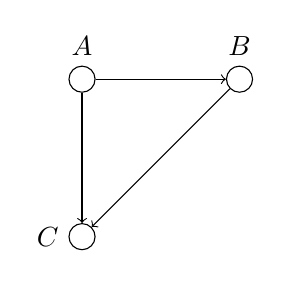
\begin{tikzpicture}[node distance=2cm]
    \node[draw,circle,label=above:$A$] (a) {};
    \node[draw,circle,right of=a,label=above:$B$] (b) {};
    \node[draw,circle,below of=a,label=left:$C$] (c) {};

    \draw[->] (a) -- (b);
    \draw[->] (a) -- (c);
    \draw[->] (b) -- (c);
\end{tikzpicture}
\caption[A directed graphical model representing the joint \acf{PDF} over the variables of~\eqref{eq:bn_bishop_ex_prod_rule_2}.]{A directed graphical model representing the joint \acf{PDF} over three variables~$A$, $B$ and~$C$ according to the decomposition of the right-hand side of~\eqref{eq:bn_bishop_ex_prod_rule_2}. Adapted from~\cite{bishop:prml}.}
\label{fig:directed_graphical_model}
\end{figure}

The above decomposition holds for any choice of the joint distribution.
We now represent the right-hand side of~\eqref{eq:bn_bishop_ex_prod_rule_2} in terms of a \emph{graphical model} as follows.
First, we introduce a node for each of the random variables $A$, $B$ and $C$, and we associate each node with the corresponding \emph{\ac{CPD}} on the right-hand side of~\eqref{eq:bn_bishop_ex_prod_rule_2}.
Second, for each \ac{CPD} we add directed edges (arrows) to the graph from the nodes corresponding to the variables on which the distribution is conditioned.
Therefore, for the factorization $p(C \given A,B)$, there will be edges from nodes $A$ and $B$ to node $C$, whereas for the factorization $p(A)$ there will be no incoming edges.

Note that the order for the factorization was arbitrary: other factorizations represent the same evidence identically.
However, if we know \apriori{} the causal relationships of the domain, we can choose the parents so that they better reflect our beliefs about the causality in the domain.

The resulting graph is shown in Fig.~\ref{fig:directed_graphical_model}.
If there is an edge going from a node $A$ to a node $B$, we say that node $A$ is a \emph{parent} of node $B$, and conversely we say that $B$ is the \emph{child} of node $A$.
We do not make any formal distinction between a node and the variable to which it corresponds, but we simply use the same symbol to refer to both (interchangeably).

We now give a few examples of conditional independence and its properties.

\begin{figure}
\centering
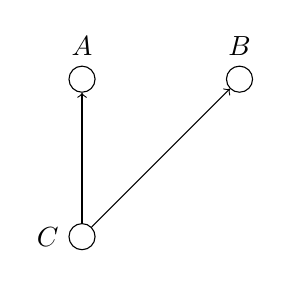
\begin{tikzpicture}[node distance=2cm]
    \node[draw,circle,label=above:$A$] (a) {};
    \node[draw,circle,right of=a,label=above:$B$] (b) {};
    \node[draw,circle,below of=a,label=left:$C$] (c) {};

    \draw[->] (c) -- (a);
    \draw[->] (c) -- (b);
\end{tikzpicture}
\caption[A directed graphical model representing the joint \acf{PDF} over the variables of~\eqref{eq:cond_indep_bishop_ex1_joint_prob}.]{A directed graphical model representing the joint \acf{PDF} over three variables~$A$, $B$ and~$C$ according to the decomposition of the right-hand side of~\eqref{eq:cond_indep_bishop_ex1_joint_prob}. Adapted from~\cite{bishop:prml}.}
\label{fig:cond_indep_bishop_ex1}
\end{figure}

As a \emph{first example} of graphical models to illustrate the concept of \emph{conditional independence}, let us consider the graph in Fig.~\ref{fig:cond_indep_bishop_ex1}.
In this case, the joint probability $p(A,B,C)$ is
\begin{equation} \label{eq:cond_indep_bishop_ex1_joint_prob}
    p(A,B,C) = p(A \given C) p(B \given C) p(C).
\end{equation}

Let us now apply the rules of probability, in particular we will \emph{marginalize} (i.e., sum out over irrelevant variables), which can be done with regard to any variable. \label{para:marginalization}
If none of the three variables is observed (see Sec.~\ref{sec:background:theory:param_learning}), then we can marginalize both sides of~\eqref{eq:cond_indep_bishop_ex1_joint_prob}, for instance with respect to~$C$, obtaining
\begin{equation*}
  p(A,B) = \sum_C p(A \given C) p(B \given C) p(C).
\end{equation*}

If, instead, we condition~\eqref{eq:cond_indep_bishop_ex1_joint_prob} on the variable~$C$, we can write the \ac{CPD} of~$A$ and~$B$ given~$C$ (conditional independence property) as
\begin{align} \label{eq:cond_indep_bishop_ex1_on_variable_C}
\begin{split}
  p(A,B \given C) &= \frac{p(A,B,C)}{p(C)} \\
                  &= p(A \given C) p(B \given C).
\end{split}
\end{align}

We can think of a graphical interpretation of~\eqref{eq:cond_indep_bishop_ex1_on_variable_C} by looking at the \emph{path} from node~$A$ to~$B$ via~$C$ in Fig.~\ref{fig:cond_indep_bishop_ex1}.
We say that~$C$ has a \emph{tail-to-tail} connection with respect to this path, because the node is connected to the tails of the two arrows, and the presence of the path connecting~$A$ and~$B$ causes these nodes to be dependent. \label{tail_to_tail}
When we condition on~$C$, the conditioned node ``blocks'' the path from~$A$ to~$B$, as a consequence~$A$ and~$B$ become (conditionally)~independent.

\begin{figure}
\centering
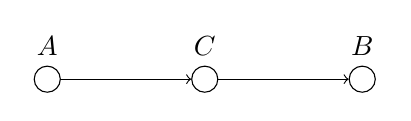
\begin{tikzpicture}[node distance=2cm]
    \node[draw,circle,label=above:$A$] (a) {};
    \node[draw,circle,right of=a,label=above:$C$] (c) {};
    \node[draw,circle,right of=c,label=above:$B$] (b) {};

    \draw[->] (a) -- (c);
    \draw[->] (c) -- (b);
\end{tikzpicture}
\caption[A directed graphical model representing the joint \acf{PDF} over the variables of~\eqref{eq:cond_indep_bishop_ex2_joint_prob}.]{A directed graphical model representing the joint \acf{PDF} over three variables~$A$, $B$ and~$C$ according to the decomposition of the right-hand side of~\eqref{eq:cond_indep_bishop_ex2_joint_prob}. Adapted from~\cite{bishop:prml}.}
\label{fig:cond_indep_bishop_ex2}
\end{figure}

As a \emph{second example}, we can consider the graph of Fig.~\ref{fig:cond_indep_bishop_ex2}.
Its corresponding joint distribution is
\begin{equation} \label{eq:cond_indep_bishop_ex2_joint_prob}
  p(A,B,C) = p(A) p(C \given A) p(B \given C).
\end{equation}

If none of the variables are observed, we can marginalize over~$C$, obtaining
\begin{align*}
\begin{split}
  p(A,B) &= p(A) \sum_C p(C \given A) p(B \given C) \\
         &= p(A) p(B \given A).
\end{split}
\end{align*}

If we condition on~$C$, using Bayes' rule~\eqref{eq:bayes} and~\eqref{eq:cond_indep_bishop_ex2_joint_prob}, we obtain the conditional independence
\begin{align*}
\begin{split}
  p(A,B \given C) &= \frac{p(A,B,C)}{p(C)} \\
                  &= \frac{p(A) p(C \given A) p(B \given C)}{p(C)} \\
                  &= p(A \given C) p(B \given C).
\end{split}
\end{align*}

We say that~$C$ is \emph{head-to-tail} with respect to the path from~$A$ to~$B$. \label{head_to_tail}
This path connects nodes~$A$ and~$B$ and makes them dependent.
If we now observe~$C$, then this observation ``blocks'' the path from~$A$ to~$B$ and we obtain the conditional independence.

\begin{figure}
\centering
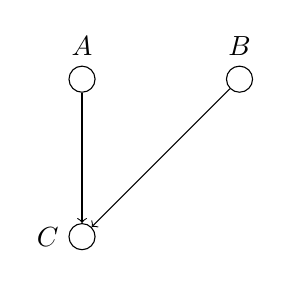
\begin{tikzpicture}[node distance=2cm]
    \node[draw,circle,label=above:$A$] (a) {};
    \node[draw,circle,right of=a,label=above:$B$] (b) {};
    \node[draw,circle,below of=a,label=left:$C$] (c) {};

    \draw[->] (a) -- (c);
    \draw[->] (b) -- (c);
\end{tikzpicture}
\caption[A directed graphical model representing the joint \acf{PDF} over the variables of~\eqref{eq:cond_indep_bishop_ex3_joint_prob}.]{A directed graphical model representing the joint \acf{PDF} over three variables~$A$, $B$ and~$C$ according to the decomposition of the right-hand side of~\eqref{eq:cond_indep_bishop_ex3_joint_prob}. Adapted from~\cite{bishop:prml}.}
\label{fig:cond_indep_bishop_ex3}
\end{figure}

As a \emph{third example}, let us consider the graph of Fig.~\ref{fig:cond_indep_bishop_ex3}.
Its corresponding joint distribution is
\begin{equation} \label{eq:cond_indep_bishop_ex3_joint_prob}
  p(A,B,C) = p(A) p(B) p(C \given A,B).
\end{equation}

If none of the variables are observed, we can marginalize both sides of~\eqref{eq:cond_indep_bishop_ex3_joint_prob} over~$C$, obtaining
\begin{align} \label{eq:cond_indep_bishop_ex3_no_vars_observed}
\begin{split}
  p(A,B) &= p(A) p(B) \cancel{\sum_C p(C \given A,B)} \\
         &= p(A) p(B).
\end{split}
\end{align}

If we condition on~$C$, using Bayes' rule~\eqref{eq:bayes} and~\eqref{eq:cond_indep_bishop_ex3_joint_prob}, we obtain the conditional independence
\begin{align*}
\begin{split}
  p(A,B \given C) &= \frac{p(A,B,C)}{p(C)} \\
                  &= \frac{p(A) p(B) p(C \given A,B)}{p(C)}.
\end{split}
\end{align*}

We say that~$C$ is \emph{head-to-head} with respect to the path from~$A$ to~$B$, because it connects to the heads of the two arrows. \label{head_to_head}
When~$C$ is not observed, it ``blocks'' that path, and the variables $A$ and~$B$ are independent, as expressed by~\eqref{eq:cond_indep_bishop_ex3_no_vars_observed}, in contrast to the two previous examples.
However, conditioning on~$C$ ``unblocks'' the path, rendering the variables~$A$ and~$B$ dependent.

Summarizing, a tail-to-tail node or a head-to-tail node leaves a path unblocked unless it is observed, in which case it blocks the path.
Instead, a head-to-head node blocks a path if it is unobserved, but once the node
(or one of its descendants\footnote{Node~$Y$ is a \emph{descendant} of node~$X$ if there is a path from~$X$ to~$Y$ in which all steps of the path follow the directions of the arrows~\cite[p.~376]{bishop:prml}.})
is observed, the path becomes unblocked.

Having examined the above instances, we shall now introduce the notion of \emph{equivalence classes} of graph structures:
two \acp{DAG}~$G$ and~$G'$ are equivalent if, for every \ac{BN} $B = (G, \theta)$, there exists another network $B' = (G', \theta')$ such that both define the same probability distribution.

\StructureLearning{} techniques, which we will describe in Sec.~\ref{sec:background:theory:structure_learning}, are able to distinguish among equivalence classes of graph structures.

This is linked with the concept of \emph{correlations} in the following sense: equivalence classes contain different correlations between the nodes of the network.

In order to be able to infer the correct correlation, i.e., to disambiguate between graph structures in the same equivalence class, it is necessary to use \emph{interventional variables}, i.e., variables which are fixed to a specific value. \label{para:interventional_vars}
We will use interventional variables in robot experiments throughout the thesis, giving an example when we describe the experimental robot setup in Ch.~\ref{chap:platform}.
The fact that robots make decisions to intervene in the world is what makes it possible to learn correlations.

\subsection{Learning the Structure of \aclp{BN}}
\label{sec:background:theory:structure_learning}

In light of the principles of developmental robotics, which is one of the motivations of this thesis (see Sec.~\ref{sec:motivation:devrob}), it is interesting to mention \StructureLearning.
Recall that, in developmental robotics, an embodied agent builds its cognition step by step, typically by incremental self-exploration of the surrounding environment, starting from a limited initial knowledge, then progressing towards the discovery of patterns and facts about the world, as time and experience advance.
In this sense, \StructureLearning{} can be loosely interpreted as the discovery of correlations in the environment.

Learning the structure of the network, $G$, is a model selection problem, where the search space contains all possible structures of \acp{DAG}, given the number of variables in the domain~\cite{pearl:1988:probabilistic}.

This can be formalized as estimating the distribution over all possible network structures~$G \in \mathcal{G}$ given the data.
Using Bayes' rule~\eqref{eq:bayes}, we can express this distribution as the product of the marginal likelihood and the prior over graph structures,
\begin{equation}
    p(G \given D) = \eta \, p(D \given G) p(G),
\end{equation}
where~$\eta = 1/p(D)$ is a normalization constant.
The prior~$p(G)$ allows to incorporate previous knowledge on possible structures.

Because the number of \acp{DAG} is super-exponential in the number of nodes~\cite{robinson:1977:dag}\footnote{%
See for example the Bayes Net Toolbox documentation (\url{http://bayesnet.github.io/bnt/docs/usage.html}), where the number of \acp{DAG} as a function of the number of nodes, $G(n)$, is given by the recurrence equation~(super-exponential in~$n$)
\begin{equation*}
G(n) = \sum_{k=1}^n (-1)^{k+1} \binom{n}{k} 2^{k(n-k)} G(n-k).
\end{equation*}%
}, it is unfeasible to enumerate all possible network structures and assign them a score, even for a low number of nodes.
This justifies the usage of heuristics to find a~(local) maximum in the structure space, approximating the full distribution.
Several methods have been proposed to approximate the distribution~$p(G \given D)$, such as:
\ac{MCMC}~\cite{madigan:1995:mcmc},
K2~\cite{cooper:1992:k2,bielza:2011:k2},
\ac{BDe}~\cite{shah:2009:pebl}.

The \ac{MCMC} algorithm~\cite{madigan:1995:mcmc} applied to \ac{BN} \StructureLearning{} generates a set of samples of possible network structures with relative frequencies that correspond to the Bayesian posterior distribution~$p(G \given D)$.
These samples can then be used to estimate the posterior probabilities of particular features of interest, marginalizing over the various structures.
Typically, implementations of this algorithm employ \MH{} sampling~\cite{giudici:2003:mcmc}.

The K2 algorithm~\cite{cooper:1992:k2,bielza:2011:k2} searches for the structure that maximizes the joint probability of structure and data, $p(G, \theta)$.
For this, it assumes a known ordering on the domain variables and that all possible structures are equally likely.
It starts from the lowest-order node and makes its way sequentially to the highest.
At each node, it first assumes that it has no parents, then it uses a greedy-search method over the K2 score~\cite{cooper:1992:k2} of the lower-order nodes to incrementally add them as its parents.
With \ac{BDe}~\cite{shah:2009:pebl}, the structure of the networks is maximized by using greedy search and simulated annealing.
In Ch.~\ref{chap:tool}, we will examine \ac{BN} \StructureLearning{} algorithms used in robot tool use affordance experiments.

\subsection{Learning the Parameters of \aclp{BN}}
\label{sec:background:theory:param_learning}

The structure of a \ac{BN} can either be provided by a human expert, or it can be learned with the methods described in the previous section.
In any case, given the structure of a \ac{BN}, the parameters~$\theta_i$ of each node can be estimated~(learned) with a Bayesian approach~\cite{heckerman:1995:learnbn}.
Then, the estimated parameters can also be updated online, permitting the incorporation of further information provided by new trials and experiments.

If a \ac{BN} has a known structure and it is fully observable~(i.e., all the variables represented by nodes are observed), the goal of parameter learning is to find the values of the \ac{BN} parameters~(in each \ac{CPD}) that maximize the (log)-likelihood of the training data.
In this case, we can use maximum-likelihood estimation.
Given a training dataset $\Sigma = \{ x_1, \dots, x_m \}$, where each $x_l = (x_{l1}, \dots, x_{ln})^\T, 1 < l < m$, is an $n$-dimensional data point corresponding to one realization~(value) of the random variable~$X_i$, and the parameter set $\theta = (\theta_1, \dots, \theta_n)$, where $\theta_i$ is the vector of parameters for the \ac{CPD} of variable~$X_i$ (represented by one node in the graph), the log-likelihood of the training dataset is a sum of terms, one for each node:
\begin{equation}
  \log L(\theta \given \Sigma) = \sum_l \sum_i \log p(x_{li} \given \parents(X_i), \theta_i).
\end{equation}

On the other hand, if the \ac{BN} is only partially observable~(i.e., some nodes are hidden or data is missing), parameter learning is~(in general) computationally intractable.
However, we can use the \EMlong~(\EM) algorithm to find a locally optimal maximum-likelihood estimate of the parameters.
If the conditional distributions and the parameter priors are conjugate, the \acp{CPD} and marginal likelihood can be computed in closed form, thus being efficient in terms of learning and inference algorithms.

\subsection{Making Inference on \aclp{BN}}
\label{sec:background:theory:inference}

Having a \ac{BN}, we can compute $p(\xinf \given \xobs)$, where~$\xobs$ is the set of observed variables, and~$\xinf$ is the set of variables on which we wish to perform an inference.
This computation is also called a query~(i.e., we query a network and as a result we obtain a response).
Usually, this is done by first converting the \ac{BN} into a tree-like structure\footnote{%
Converting a \ac{BN} graph into a tree is an operation that involves several computational steps.
For a detailed explanation see, for example, \cite[p.~416]{bishop:prml}.}, % end footnote
and then applying the \emph{\jtree{}} algorithm~\cite{lauritzen:1988:jtree,huang:1996:jtree,bishop:prml} in order to compute the queried distribution of interest.
The advantage of the \jtree{} algorithm is that of avoiding to work directly with the joint distribution of the variables considered, relying instead on factorization properties.

Importantly, for performing inference it is not necessary to know all the values of all the variables.
This entails that a query can combine any combination of the nodes (e.g., any combination that uses object features, actions and effects, as we will see in the affordances applications in Sec.~\ref{sec:background:previous_works}) either as observed variables or as the desired~(inferred) output.

Based on this probabilistic machinery, we can now use an affordance knowledge \ac{BN} to answer questions such as ``which is the best action to achieve an effect?'' or ``which effect will be obtained by exerting this action on this object?'', simply by computing the appropriate distributions.
For instance, predicting the effects of an observed action~$a_i$ given the observed features~$o_j$ can be performed from the distribution $p(E \given A=a_i, O=o_j)$.

The advantage of using \acp{BN} is that their expressive power allows the marginalization over any set of variables given any other set of variables.
For instance, referring to the diagram of Fig.~\ref{fig:aff_models_intro:montesano} which depicts the computational model of affordances by Montesano~\cite{montesano:2008}, one can extract different types of information~(i.e., perform different types of queries) from a previously-trained network, such as:
\begin{description}
\item[effect prediction] Given the motor action~$A$ executed by the robot and its target object~$O$, compute the distribution of the resulting physical effects: $p(E \given A,O)$;

\item[planning] Given the target object~$O$ and the (desired) physical effect~$E$, compute the appropriate motor action:
    \begin{equation*}
      A^{*} = \argmax_{A} p(A \given O,E);
    \end{equation*}

\item[object properties] Given the target object~$O$, compute the distribution of its possible physical effects: $p(E \given O)$;

\item[action properties] Given the motor action~$A$, compute the distribution of possible resulting physical effects: $p(E \given A)$.
\end{description}

\section{Previous Works}
\label{sec:background:previous_works}

In this section, we outline some previous works in the literature which are related to the broad scope of the thesis.
Explaining these works is useful to understand the contributions of the next chapters, where we will also provide chapter-specific summaries of the related works about particular topics.

What the works described below have in common is that they tackle the challenges associated with having autonomous robots operate in human-centered, unstructured environments.
To do that, they propose
(i)~to equip robots with the capability of building a \emph{model of the environment} surrounding them from autonomous exploration;
(ii)~to incorporate~(in such a model of the environment) elements such as physical \emph{objects} present in a scene, their affordances, and possibly the information expressed by human agents by performing physical \emph{actions} or body gestures;
(ii)~to use such a model for making sense or finding meaning~(in other words, to do \emph{reasoning}) about the environment.

This possibility of robots reasoning about their environment has several applications: prediction of the future, imitation of another agent, planning of complex actions that require multiple sub-actions, provision of feedback to humans when doing shared \hr{} collaboration tasks.

We now proceed in citing the previous works, categorized according to their main focus or topic.

\subsection{Reasoning about Objects}
\label{sec:background:previous_works:montesano}

In the previous chapter we have mentioned some advantages obtained by incorporating object affordances in cognitive robotic systems.
The concept of affordances is applicable to autonomous robots and has influenced many robotic studies and models, specifically because
(i)~affordances depend on perceptual and motor capabilities of the agent~(e.g., whether the robot is mobile or not, how tall it is, whether it has arms, actuators, etc.);
(ii)~affordances suggest action possibilities to the agent from direct perception, thus providing a means to predict the consequences of physical actions~(e.g., accomplish a given goal in a novel situation, as in the coffee example of p.~\pageref{coffee_example}).

We can summarize the advantages as follows:
\begin{enumerate}
    \item affordances can be \emph{learned} by a robot that explores different actions exerted on the environment (e.g., on the objects present in the environment) autonomously, or semi-autonomously;

    \item after learning, the acquired knowledge can be used for \emph{reasoning} (e.g., to perform inference about object and action properties);

    \item affordances are \emph{robust} in the sense that they can use incomplete data or limited data.
\end{enumerate}

The above aspects are relevant because modeling all the possible world interactions of a robot is unfeasible~(see Sec.~\ref{sec:motivation:affordances}), thus learning from experience is required.
In turn, this poses the challenge of collecting a large amount of experiments or training data, which can be partially mitigated by learning affordance models that perform adequately with only limited data.

The idea of using object affordances for supporting robot capabilities such as scene understanding, reasoning and learning, has been proposed by several authors since the mid-2000s~\cite{fitzpatrick:2003:icra,lopes:2005:smcb,moratz:2008} with different aims and motivations.
In perceiving human activities, object affordances can be used to infer the action executed by a user just by observing the resulting effect~\cite{kozima:2002:epirob,montesano:2008}.
This knowledge can then be used to make a robot provide feedback, or to imitate the human action with skill transfer~\cite{kozima:2002:epirob,lopes:2005:smcb,lopes:2007:iros,lopes:2007:smcb}, or to actively aid the human towards realizing a shared collaborative plan~\cite{lallee:2013:iros,jiang:2013:cvpr}.
Thill~\cite{thill:2013:jneubiorev} published a review of computational models of affordances inspired by the mirror neuron system.
More recently, a survey about the role of affordances in psychology, neuroscience, and robotics was published~\cite{jamone:2016:tcds}, followed by a comprehensive taxonomy of approximately~150 computational models of affordances in the robotics literature~\cite{zech:2017:ab}.

In this section, we focus on the work by Montesano~\cite{montesano:2008,montesano:2010:bookchap}, which is the starting point behind the contributions presented in this thesis.

\begin{figure}
\centering
\subfloat[][Humanoid robot in its workspace with a table and some objects.]
{\includegraphics[width=0.546\textwidth]{montesano_setup} } \quad
%
\subfloat[][Objects being perceived and visually segmented by vision algorithms.]
{\includegraphics[width=0.364\textwidth]{montesano_shapeExample} }
\caption[Experimental setup of~\cite{montesano:2008}.]{Experimental setup of~\cite{montesano:2008}. In this work, a robot learns object affordances by autonomous exploration of colorful toys on a table; affordances are modeled as relationships between actions, objects and effects.}
\label{fig:montesano_setup}
\end{figure}

That work is influential in the cognitive robotics community, because it shows a computational model of affordances that is able to account for multiple possible affordances present in a robot's environment in a principled and probabilistic way, as opposed to assuming the existence of only one pre-defined affordance~(e.g., liftability).
In other words, this model is capable of learning multiple affordances present in the environment, or multiple possibilities offered by the objects perceived by the agent.
Computationally, it achieves this by using a \ac{BN} with a structure that encodes relations between motor actions, object features and resulting effects, as depicted in Fig.~\ref{fig:aff_models_intro:montesano}.

In a self-exploration manner (see Sec.~\ref{sec:motivation:devrob}), the Baltazar humanoid robot~\cite{lopes:2004:baltazar} tries out different motor actions onto different physical objects and records the observed effects, as shown in Fig.~\ref{fig:montesano_setup}.
Then, it learns the relations between the random variables involved (i.e., the variables pertaining to actions, object features and effects).
The actions are pre-defined tapping motions performed with the end effector, from four different directions.
The object features are (discretized) quantities related to size, shape, and color of objects extracted from vision.
The effects are the (discretized) physical displacements of the objects being moved on a tabletop, and the (discretized) durations of the contacts acquired with tactile sensors.
Data is discretized by using $k$-means clustering~\cite{lloyd:1982:kmeans} in order to train the \ac{BN} efficiently.

By repeating the exploration procedure several times, the robot acquires a set of~$N$ samples
\begin{equation}
    D = \{ y^{1:N} \},
\end{equation}
where the lower-case letter~$y$ represents the possible realizations~(i.e., values) of the random variable indicated by the upper-case letter~$Y$ (see Sec.~\ref{sec:background:theory:probability}).
Then, the set of nodes in a network,~$Y$, includes all of its variables, i.e., the ones representing robot actions~($A$), object features~($O$) and resulting effects~($E$), as follows:
\begin{equation}
    Y = \{ A, O_1,\dots,O_{n_O}, E_1,\dots,E_{n_E} \}.
\end{equation}

For the sake of this summary, let us assume for simplicity that the structure of the \ac{BN} is known, i.e., that we know the dependencies between the variables in~$Y$.

Given the (discrete) representation of actions, object features and effects, the authors use a \emph{multinomial distribution} and its corresponding conjugate, the Dirichlet distribution, to model the \acp{CPD} $p \left( Y_i \biggiven Y_{\parents(Y_i)}, \theta_i \right)$ and the corresponding parameter priors $p(\theta_i)$, respectively.
Let~$\mathcal{Y}_i$ and~$\mathcal{Y}_{\parents(Y_i)}$ indicate the range of values of random variables~$Y_i$ and the range of values of the parent nodes of~$Y_i$, respectively.
Assuming independence between the samples in~$D$, the marginal likelihood for the random variable~$Y_i$ and its parents given~$D$~(\cite{heckerman:1995:learnbn}) is:
\begin{align*}
p \left( y_i^{1:N} \biggiven y_{\parents(Y_i)}^{1:N} \right) &= \int \prod_{n=1}^n p \left( y_i^N \biggiven y_{\parents(Y_i)}^n, \theta_i \right) p(\theta_i) \, d\theta_i \\
 &= \prod_{j=1}^{|\mathcal{Y}_i|} \frac{\Gamma(\alpha_{ij})}{\Gamma(\alpha_{ij}+N_{ij})} \prod_{k=1}^{|\mathcal{Y}_{\parents(Y_i)}|} \frac{\Gamma(\alpha_{ijk}+N_{ijk})}{\Gamma(\alpha_{ijk})},
\end{align*}
where~$N_{ijk}$ counts the number of samples in which~$Y_i = j$ and~$Y_{\parents(Y_i)} = k$, $N_{ij} = \sum_k N_{ijk}$ and~$\Gamma$ represents the gamma function.
The \emph{pseudo-counts}~$\alpha_{ijk}$ denote the Dirichlet hyper-parameters of the prior distribution of~$\theta_i$ and $\alpha_{ij} = \sum_k \alpha_{ijk}$.
The marginal likelihood of the data is simply the product of the marginal likelihood of each node,
\begin{equation}
    p(D \given G) = p(Y^{1:N} \given G) = \prod_i p \left( y_i^{1:N} \biggiven y_{\parents(Y_i)}^{1:N} \right),
\end{equation}
where we have made explicit the dependency on the graph structure,~$G$.

One of the characteristics of Montesano's computational model of affordances is that it relies on discrete quantities being computed~(by a clustering algorithm) and passed as input to the \ac{BN}, rather than on the raw continuous-valued variables themselves.
In an extention work, Osório relaxes this assumption~\cite{osorio:2010:iros} in order to use the continuous values directly, by employing \acp{GMM} to represent the perceived visual features.
Results from a simulated environment suggest that continuous values can help \acp{BN} when data is noisy and when plenty of training data is available.
However, the practical applicability of this approach on real robots is problematic because of its
computational cost: the proposed solution uses the \EMlong~(\EM) algorithm, whose execution time is much slower than the one of Montesano's discrete \ac{BN} nodes.

Also, Montesano's model examines the possibilities afforded by \emph{one object}~at a time to the agent~(e.g., a ball affords high rollability).
In Ch.~\ref{chap:tool} we will extend the model in the context of \emph{tool use} affordances, meaning that, with exploration, the robot will learn to reason about two objects at a time, to be used as a tool and as an affected object, respectively~(e.g., a hammer and a nail).

\subsection{Affordances and Language}
\label{sec:background:previous_works:aff_language}

We have mentioned that robot affordances can help understanding a user's intention by recognizing the action performed by them.
Additionally, some works have used the concept of \emph{sensor fusion} to build \emph{multimodal affordances}, for example incorporating human language in addition to objects, where different modalities complement each other.

One of the first papers in this category is the one by Moratz~\cite{moratz:2008}, where linguistic instructions from a human to a robot are grounded in the affordances of objects present in a scene.
This system employs a robot object recognition system composed with a laser range finder, making use of an affordance-informed visual algorithm~(relating object shapes to object functionalities in a way pre-defined by the experimenter).
As a result, the system can be used to instruct a robot verbally, so that words relating to the affordances are mapped to the objects allowing the robot to choose the objects to use.
Notably, this setup requires a pre-defined set of known objects and of the rules associating affordances to objects.
Also, this approach does not exploit the information contained in nonverbal language, such as human gestures and movements.

\begin{figure}
    \includegraphics[width=0.9\textwidth]{salvi_scheme}
    \caption[Experimental setup of~\cite{salvi:2012:smcb}.]{Experimental setup of~\cite{salvi:2012:smcb}. In this work, which extends~\cite{montesano:2008}, a robot learns associations between \emph{spoken words} and object affordances~(where affordances are modeled as the relationships between actions, object features, effect features).}
    \label{fig:salvi_setup}
\end{figure}

A system with less stringent assumptions is the one by Salvi~\cite{salvi:2012:smcb}, whose experimental setup is shown in Fig.~\ref{fig:salvi_setup}.
In this work, building upon Montesano's model~(see Sec.~\ref{sec:background:previous_works:montesano}), object affordances are used to associate human words to the actual action, object and effect that they refer to.
Computationally, \acp{BN} are used, serving to learn \wordsmeanings{} associations.
This knowledge is then used together with spoken instructions for removing ambiguities during interactions with humans, for example permitting to command the robot to perform tasks.
We will expand upon the system by Salvi in Ch.~\ref{chap:gestures}.

Another work relating affordances and language is~\cite{celikkanat:2015:tamd}, which models the co-occurrence of actions, object information and language with a \emph{concept web} based on \acp{MRF}.
During operation, if partial information is available~(e.g., only the visual object information or the corresponding words), the corresponding affordance concepts previously learned are also activated.

\subsection{Reasoning about Human Actions}
\label{sec:background:previous_works:reasoning_about_human_actions}

Up to now, we have mentioned a number of works about robots that explore their environment, they operate on it~(e.g., using their limbs), and they build a cognitive model of the environment that takes into account the physical objects and the afforded actions.
Even though some of the works considered language, which is a human trait, the human dimension was not prominent in a physical or visual sense, meaning that the cognitive model used by the robot did not have any explicit representation of human users~(e.g., their location, their state, their physical action).
However, a growing line of research \emph{does} tackle this aspect, incorporating advances from other disciplines~(e.g., human activity recognition, machine learning and computer vision~\cite{aggarwal:2011}) onto robots.

Thus, we now list some works about autonomous robots possessing cognitive reasoning algorithms about environment objects \emph{and the humans} surrounding them.
This list is not exhaustive, but it is useful to understand the contributions of the next chapters.

\begin{figure}
\centering
\includegraphics[width=0.9\textwidth]{aloimonos_eggplant}
\caption{Sequence of frames of a cutting action, reproduced from~\cite{pastra:2012:rstb}.}
\label{fig:minimalist_eggplant}
\end{figure}

Pastra and Aloimonos~\cite{pastra:2012:rstb} propose a ``minimalist grammar of action'' for robot cognition, linking the two aspects of language and action together.
That work is motivated by the biological evidence that both language and action are organized in a hierarchical, compositional way, and that the neural locus for composing their mechanisms is shared in Broca's area~\cite{pulvermuller:2005:broca}.
For example, Fig.~\ref{fig:minimalist_eggplant} shows a human person cutting an eggplant.
In order to do that, the person uses some prior knowledge and performs a sequence of low-level motor actions~(e.g., reaching for a knife tool, positioning the knife over the vegetable, exerting a vertical force to cut the vegetable, etc.), resulting in a high-level action~(e.g., cutting the vegetable).
In short, the proposed ``grammar'' is a formal, tree-like specification of actions with a biological human base.
This specification allows the development of generative computational models for action in the motor and visual space, by deploying a software component of a semantic memory~(i.e., the general human knowledge accumulated with experience) called the PRAXICON~\cite{pastra:2008:praxicon,mavroeidis:2016:praxicon}.
Indeed, this integration has been performed on a humanoid robot during the POETICON++ project\footnote{\url{http://www.poeticon.eu/} \label{footnote:poeticon++}}, and it will be described in detail in Ch.~\ref{chap:poeticon++_case_study}.

\begin{figure}
\centering
\includegraphics[width=0.9\textwidth]{wang2013-robot_table_tennis}
\caption{Tennis-playing robot, from~\cite{wang:2013:ijrr}.}
\label{fig:robot_table_tennis}
\end{figure}

In~\cite{wang:2013:ijrr}, a group from the Technical University of Darmstadt shows an example of a robotic system capable of recognizing and \emph{anticipating} a human's movements.
This system, shown in Fig.~\ref{fig:robot_table_tennis}, is capable of playing table tennis against a human opponent, using vision, control and machine learning.
It uses Gaussian Processes~\cite[p.~303]{bishop:prml}, finding a latent state representation of noisy and high-dimensional observations of human movement, at the same time capturing the dynamics of the motor task being considered.
Online approximate inference permits to anticipate the target position of the tennis ball~(i.e., the table region where the ball will fall) when the opponent performs the actual strike.
The predicted intention is then used to select the optimal robot hitting type~(e.g., forehand, middle, backhand strike).
This system requires specialized hardware, such as Gigabit Ethernet camera sensors with~200 frames per second.

\begin{figure}
\centering
\includegraphics[width=0.9\textwidth]{wu2016watch-bot}
\caption[The Watch-n-Patch assistive robot system, reproduced from~\cite{wu:2016:icra}.]{The Watch-n-Patch assistive robot system, reproduced from~\cite{wu:2016:icra}. After spotting an unusual or incomplete action, the robot signals the information to the human user with a laser pointer.}
\label{fig:watchbot}
\end{figure}

The interest in vision techniques aimed at understanding human activity from videos has also grown~(e.g., using YouTube or other large video datasets).
In~\cite{wu:2015:cvpr}, a group by Cornell University propose a method to decompose complex events into simpler actions with video segmentation, and then learn the sub-action dynamics using an unsupervised graphical model, based on \acp{CRF} over Kinect~v2 data.
In~\cite{wu:2016:icra}, they then demonstrate how Watch-n-Patch\footnote{\url{http://watchnpatch.cs.cornell.edu/}}, an assistive robot with such a previously-trained system on board, can be useful not only to monitor daily human activities, but also to actively remind users of steps and pieces that they might forget in their typical activity sequences.
For example, they do that by using a laser pointer to indicate a ``forgotten'' object~(e.g., a milk carton) that was not handled appropriately after usage~(e.g., it was not put back in the fridge).

Koppula~\cite{koppula:2016:pami} consider the problems of detecting and anticipating human activities by combining complex full-body human trajectories, robot trajectories and object affordances knowledge in a graphical model based on \acp{CRF}.
That work shows that this kind of model can improve detection and anticipation over human action datasets.
The object affordances part in that model consists of a prior grounding specified by the programmer, assigning categories like ``drinkable'', ``pourable'', ``reachable'' to \actobj{} and \objobj{} relations, where the object features are \ac{SIFT}~\cite{lowe:1999:sift}.

The above ideas have also been explored in psychology, for example by Sciutti~\cite{sciutti:2015:fpsyg}, where the authors propose a model to make humanoid robots anticipate human partners' intentions, based on actively engaging humans in face-to-face interation and measuring the subtle kinematic movement signals that emerge.

\begin{figure}
\centering
\includegraphics[width=0.6\textwidth]{chu_hri2016_curi}
\caption{A human guides a robot while it tries motor actions onto world objects to learn their affordances, from~\cite{chu:2016:hri}.}
\label{fig:chu_hri2016_curi}
\end{figure}

In~\cite{chu:2016:hri}, a group from Georgia Tech analyzes the impact of providing human guidance to a robot while it explores the environment and learns affordances~(see Fig.~\ref{fig:chu_hri2016_curi}), as opposed to having the robot learn them autonomously, like the approaches that we described so far.
In a controlled scenario with four household objects that a humanoid robot manipulates with different action parameters, they conclude that a mixed approach (i.e., partially human-guided, partially using self-exploration biased by information previously provided from human teachers) is effective for learning the affordances, requiring fewer interactions than other modalities.
A strong limitation of this approach is that it considers affordances as binary values~(i.e., does an object offer a specific affordance or not?) rather than probabilistically.
As previously mentioned, a probabilistic representation is key in modeling the inherent noise in uncontrolled, human environments.

\bigskip

In this chapter, we have provided the fundamental information needed to understand the contributions of the thesis in the next chapters.
Specifically,
we have gone through some theory~(\aclp{BN}) and
we have listed relevant works related to the broad scope of the thesis.
